% 0164(본책 29쪽) — 직선 ax−by+c=0 의 그래프(기울기 음수·y절편 양수·x절편 양수). 스캔 그림이라 TikZ 로 다시 그림.
% 라벨은 원문 그대로 O·x·y 만. 눈금·수치는 원문에 없다.
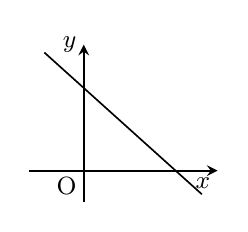
\begin{tikzpicture}[scale=0.5, line width=0.5pt]
  \draw[->, >=stealth, line width=0.7pt] (-1.4,0) -- (3.4,0) node[below left=-1pt, font=\small] {$x$};
  \draw[->, >=stealth, line width=0.7pt] (0,-0.8) -- (0,3.2) node[left=-1pt, font=\small] {$y$};
  \draw[line width=0.6pt] (-1.0,3.0) -- (3.0,-0.6);
  \node[below left=-1pt, font=\small] at (0,0) {$\mathrm{O}$};
\end{tikzpicture}
